\documentclass[french, 12pt, a4paper]{article}
\usepackage[top=3cm, bottom=3cm, left=3cm, right=3cm]{geometry}
\usepackage[utf8]{inputenc}
\usepackage[T1]{fontenc}
\usepackage{babel}
\usepackage{parskip}
\usepackage{titlesec}
\usepackage{amsmath}
\usepackage{amssymb}
\usepackage{mathtools}
\usepackage{xcolor}
\usepackage{bbm}
\usepackage{soul}
\usepackage{xifthen}
\usepackage{bm}
\usepackage{graphicx}
\usepackage{amsfonts}
\usepackage{float}

% =======================================================

\numberwithin{equation}{subsection}

\titlespacing\section{0pt}{20pt}{0pt}
\titlespacing\subsection{0pt}{20pt}{0pt}

\renewcommand{\vec}[1]{\underline{#1}}

\newcommand{\tenstwo}[1]{\underline{\underline{#1}}}
\newcommand{\tp}{\kern 2pt {}^{T\!\!}}
\newcommand{\roggt}{\underline{\text{rot}}}
\newcommand{\set}[1]{\left\lbrace #1\right\rbrace}
\newcommand{\norme}[1]{\left\Vert #1\right\Vert}

\newcommand{\seminorme}[1]{| #1 |}

\newcommand{\tendvers}{\xrightarrow[n \to \infty]{}}
\newcommand{\sdots}{\makebox[1em][c]{.\hfil.\hfil.}}
\newcommand{\et}{\text{ et }}

\newcommand{\ouvert}{\Omega}
\newcommand{\ferme}{{\overline\Omega}}
\newcommand{\frontiere}{{\partial\Omega}}

\newcommand{\ps}[2]{\left \langle #1,#2 \right \rangle}

\renewcommand{\arraystretch}{1.5}

\let\oldforall\forall
\renewcommand{\forall}{\ \oldforall}

\DeclareMathOperator{\tr}{trace}
\DeclareMathOperator{\grad}{grad}
\DeclareMathOperator{\divv}{div}
\DeclareMathOperator{\rot}{rot}

\mathtoolsset{showonlyrefs}

%\arraycolsep=15.4pt

\def\bal#1\eal{\begin{align}#1\end{align}}

\renewcommand{\phi}{\varphi}
%\renewcommand{\arraystretch}{1.5}

\newcommand{\tenscont}{\tenstwo \sigma}

\newcommand{\pr}[1][]{
    \ifthenelse {\isempty{#1}}
        {\frac{\partial}{\partial r}}
        {\frac{\partial^#1}{\partial r^#1}}
}

\newcommand{\pt}[1][]{
    \ifthenelse {\isempty{#1}}
        {\frac{\partial}{\partial \theta}}
        {\frac{\partial^#1}{\partial \theta^#1}}
}

\newcommand{\pz}[1][]{
    \ifthenelse {\isempty{#1}}
        {\frac{\partial}{\partial z}}
        {\frac{\partial^#1}{\partial z^#1}}
}

\begin{document}

% ==============================================================================

\begin{center}
{\Large\textbf{4M054 : Mise en oeuvre des éleménts finis}}

{\large\textbf{Projet 2018/2019}}

\smallskip
{\large{David Frenkiel (3770971)}}

{\large{28/04/2019}}

\end{center}
\vspace{20pt}

% ==============================================================================

\section*{Question 1}

\paragraph{Exécuter le code :}
\begin{verbatim}
  ./question.sh 1a data/maillages/maillage1_1.txt
  ./question.sh 1b data/maillages/maillage1_1.txt
\end{verbatim}

\paragraph{Le code se trouve dans}
\begin{verbatim}
  questions/q1b_afficher_maillage.py
\end{verbatim}

\begin{figure}[H]
\centering
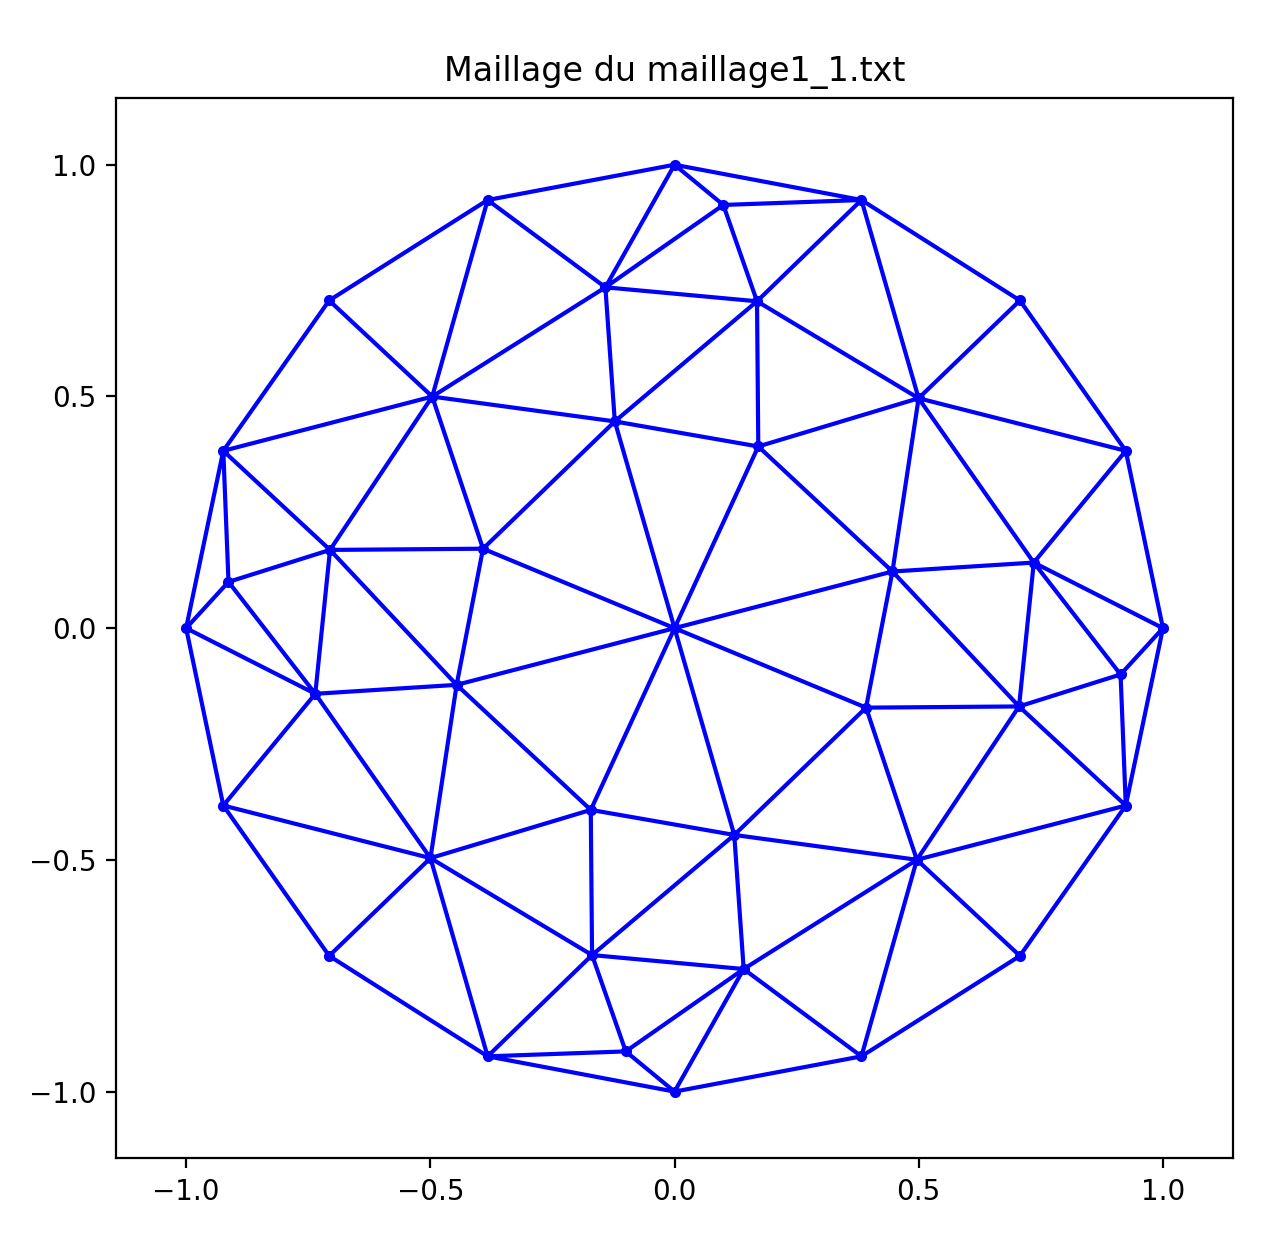
\includegraphics[scale=0.5]{figure_1b.png}
%\caption{Write some caption here}
\end{figure}

% ==============================================================================

\section*{Question 2}

\paragraph{Exécuter le code :}
\begin{verbatim}
  ./question.sh 2 data/maillages/maillage3_3.txt
\end{verbatim}

\paragraph{Le code se trouve dans}
\begin{verbatim}
  questions/q2_afficher_maillage_bord.py
\end{verbatim}

\begin{figure}[H]
\centering
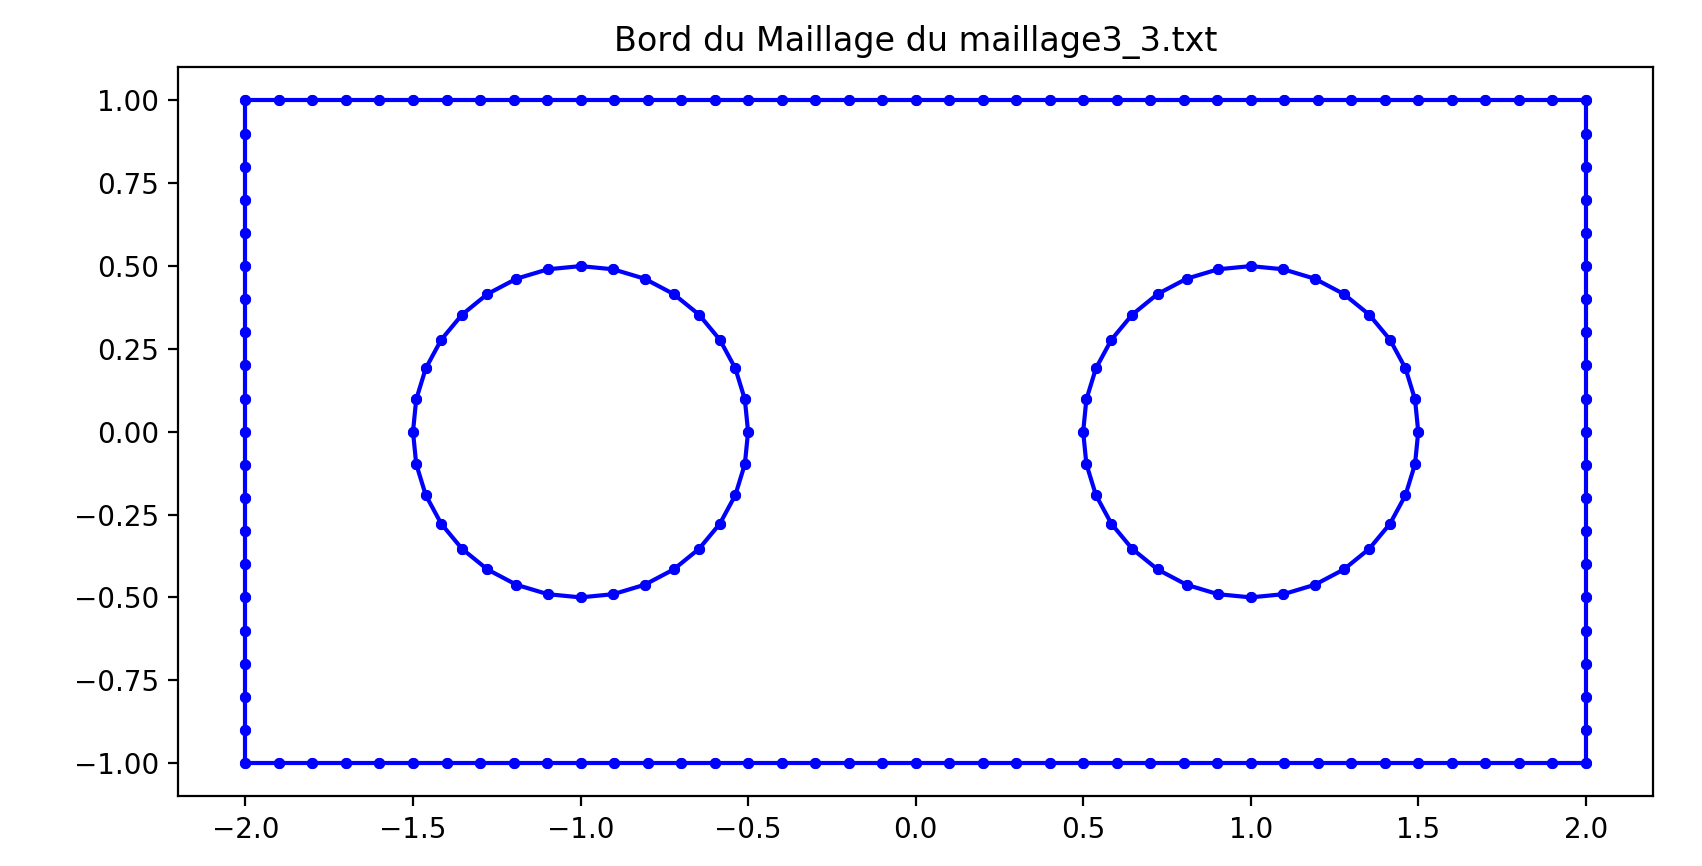
\includegraphics[scale=0.6]{figure_2.png}
\end{figure}

% ==============================================================================

\section*{Question 3}

On aimerait écrire le problème suivant sous forme variationnelle :

\[
\begin{dcases}
-\Delta u = f \text{ dans } \ouvert \\
u = 0 \text{ sur } \Gamma \\
\text{où } f \in C^\infty(\mathbb{R}^2)
\end{dcases}
\]

On suppose que $u \in C_0^2(\ouvert)$ et on se donne $v \in C_0^1(\ouvert)$.
Ensuite on multiplie l'égalité par $v$ et on l'integre. Cela nous donne
\[
-\int_\ouvert v \Delta u \; dx = \int_\ouvert vf \; dx
\]

Comme $u \in C_0^2(\ouvert)$ et $v \in C_0^1(\ouvert)$ on peut donc se
servir d'une formule de Green, ce qui nous améne à
\[
\int_\ouvert \nabla v \cdot \nabla u \; dx
- \int_\Gamma v \nabla u \cdot n \; d\sigma = \int_\ouvert vf \; dx
\]

Comme $v$ est nulle sur $\Gamma$ on arrive finalement à
\[
\int_\ouvert \nabla v \cdot \nabla u \; dx = \int_\ouvert vf \; dx
\]

Comme $C_0^1(\ouvert)$ est dense dans $H_0^1(\ouvert)$ on suppose maintenant
que $u \in H_0^1(\ouvert)$. Par passage à la limite on en tire la formulation
variationnelle suivante :

\[
\begin{dcases}
\text{Trouver } u \in H_0^1(\ouvert) \text{ telle que} \\
a(u, v) = \ell(v) \forall v \in H_0^1(\ouvert)
\end{dcases}
\]

Où
\begin{align}
a(u, v) &= \int_\ouvert \nabla v \cdot \nabla u \; dx \\
\ell(v) &= \int_\ouvert vf \; dx
\end{align}

Pour démontrer la coércivité de $a(u, v)$ on note tout d'abord que, par l'inégalite
de Poincaré, il existe une constante $C > 0$ telle que
\[ \norme{u}^2_{H^1(\ouvert)} \le C \norme{\nabla u}^2_{L^2(\ouvert)}
   \forall u \in H_0^1(\ouvert) \]

Il s'ensuit que
\begin{align}
a(u, u) &= \int_\ouvert \nabla u \cdot \nabla u \; dx = \norme{\nabla u}^2_{L^2(\ouvert)} \\
& \ge \frac{1}{C} \norme{u}^2_{H^1(\ouvert)}
\end{align}

On a ainsi démontré la coércivité de $a$.

\paragraph{Exécuter le code :}
\begin{verbatim}
  ./question.sh 3 data/maillages/maillage2_2.txt
\end{verbatim}

\paragraph{Le code se trouve dans}
\begin{verbatim}
  questions/q3_resoudre_probleme_poisson.py
\end{verbatim}

\begin{figure}[H]
\centering
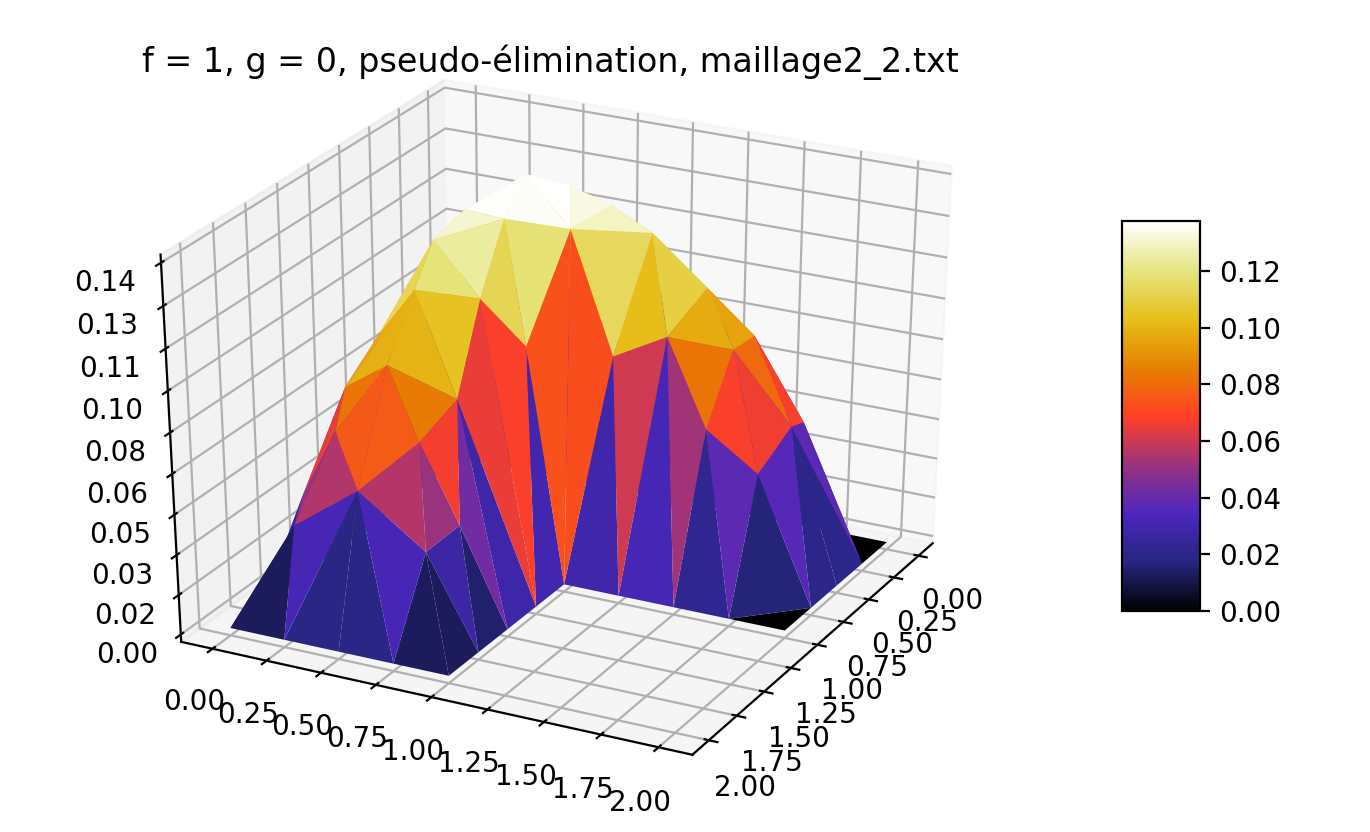
\includegraphics[scale=0.6]{figure_3.png}
\end{figure}

% ==============================================================================

\section*{Question 4}

On aimerait resoudre analytiquement l'équation de Poisson aux conditions de
Dirichlet homogène dans le disque unité ($\Omega = \{x \in \mathbb{R}^2, |\bm x| < 1\}$).
On cherche $u \in C^2(\ouvert)$ telle que
\[
\begin{dcases}
-\Delta u = 1 \text{ dans } \Omega \\
u = 0 \text{ sur } \Gamma
\end{dcases}
\]

Étant donné la symétrie circulaire du domaine on peut se servir du laplacien
en coordonnées polaires :
\[
\Delta f(r, \theta) =
\frac{1}{r} \pr \left(r \frac{\partial f}{\partial r} \right)
+ \frac{1}{r^2} \frac{\partial^2 f}{\partial \theta^2} \right)
\]

En plus, étant donné la symétrie circulaire de $u$ sur la frontière on peut
supposer que $u$ ne dépend pas de $\theta$. Il faut donc resoudre l'équation
differentielle suivante :
\[
-\frac{1}{r} \pr \left(r \frac{\partial u}{\partial r} \right) = 1 \\
\text{, où } u = 0 \text{ sur } \Gamma
\]

Cette équation se resoudre facilement en l'intégrant 2 fois :

\[ \frac{1}{r} \pr \left(r \frac{\partial u}{\partial r} \right) &= -1 \]
\[ \Rightarrow \pr \left(r \frac{\partial u}{\partial r} \right) &= -r \]
\[ \Rightarrow r \frac{\partial u}{\partial r} &= -\frac{1}{2} r^2 + A \]
\[ \Rightarrow \frac{\partial u}{\partial r} &= -\frac{1}{2} r + \frac{A}{r} \]
\[ \Rightarrow u &= -\frac{1}{4} r^2 + A \log r + B \]

Comme on cherche une solution dans $C^2(\ouvert)$ il faut que $A$ soit $0$. Donc
\[ u &= -\frac{1}{4} r^2 + B \]

Et comme $u(1) = 0$, il en resulte que $B = \frac{1}{4}$. On a alors la solution suivante :
\[ u(r) &= \frac{1}{4} - \frac{1}{4} r^2 \]

Et donc en coordonnées cartésienne :
\[ u(\bm x) &= \frac{1 - |\bm x|^2}  {4} \]

\paragraph{Exécuter le code :}
\begin{verbatim}
  ./question.sh 4
\end{verbatim}

\paragraph{Le code se trouve dans}
\begin{verbatim}
  questions/q4_verifier_solution_poisson_disque.py
\end{verbatim}

\begin{figure}[H]
\centering
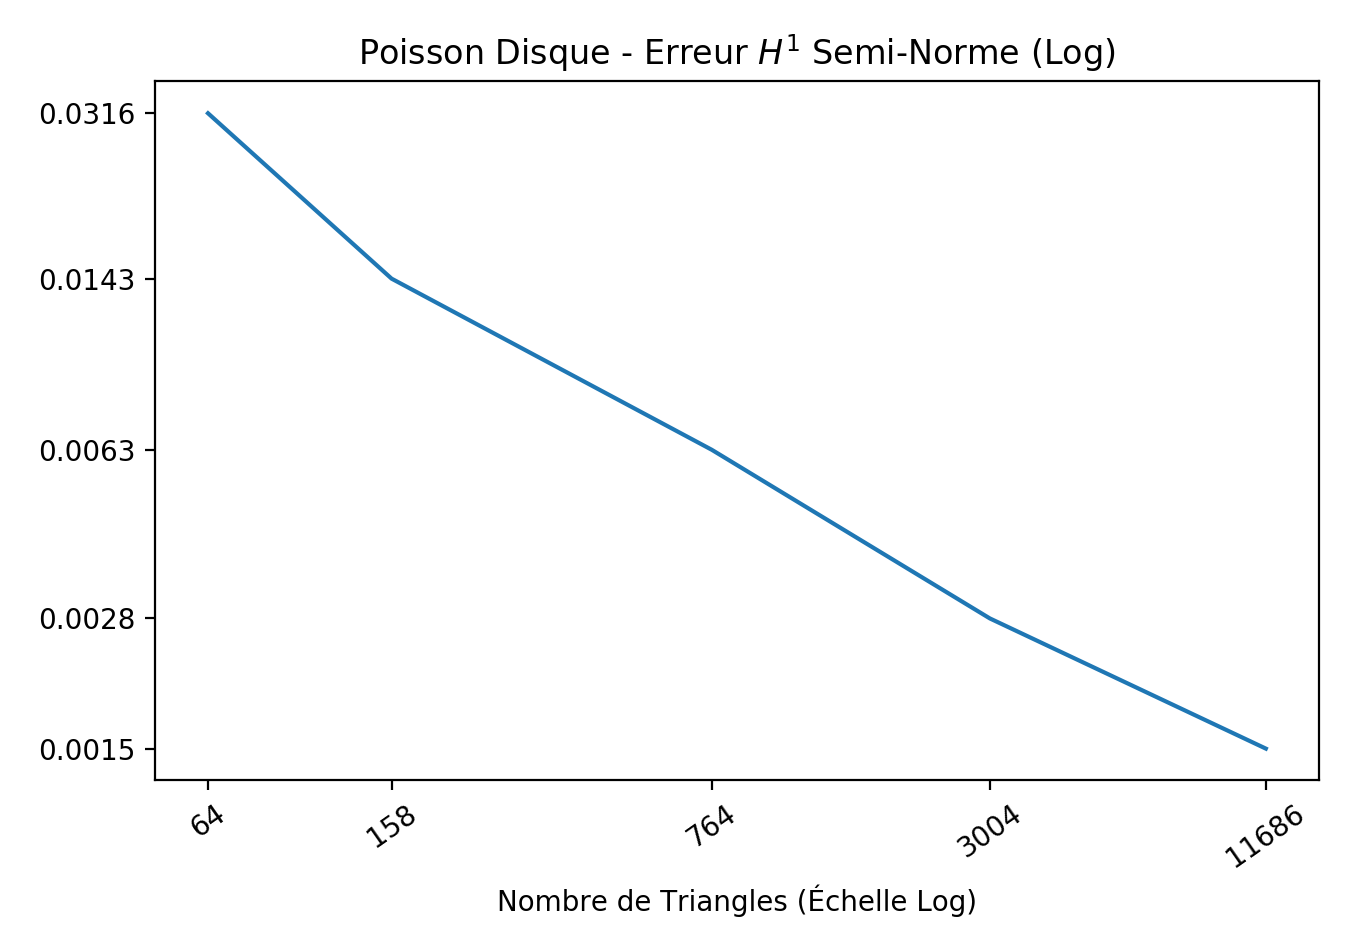
\includegraphics[scale=0.6]{figure_4.png}
\end{figure}

% ==============================================================================

\section*{Question 5}

\paragraph{Exécuter le code :}
\begin{verbatim}
  ./question.sh 5 data/maillages/maillage3_2.txt
\end{verbatim}

\paragraph{Le code se trouve dans}
\begin{verbatim}
  questions/q5_resoudre_probleme_poisson_tilde.py
\end{verbatim}

\begin{figure}[H]
\centering
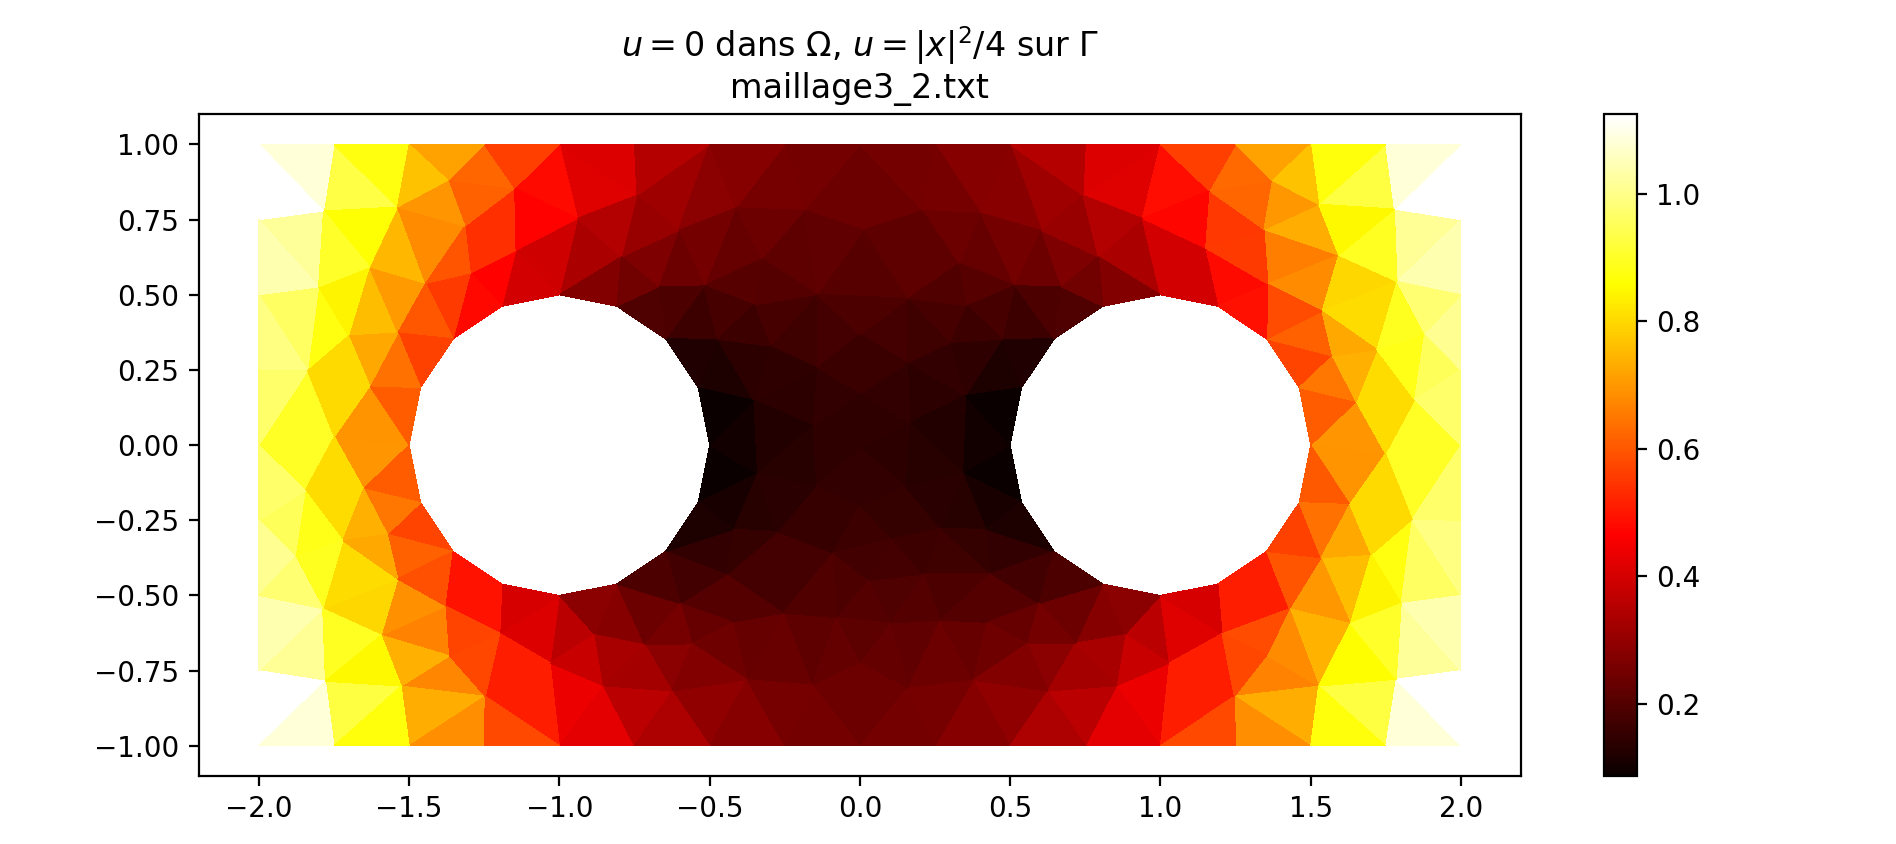
\includegraphics[scale=0.6]{figure_5.png}
\end{figure}

% ==============================================================================

\section*{Question 6}

Veuillez noter que dans la visualisation $h$ est définie comme la longueur de
l'arête le plus long du maillage.

\paragraph{Exécuter le code :}
\begin{verbatim}
  ./question.sh 6
\end{verbatim}

\paragraph{Le code se trouve dans}
\begin{verbatim}
  questions/q6_verifier_solution_poisson_tilde.py
\end{verbatim}

\begin{figure}[H]
\centering
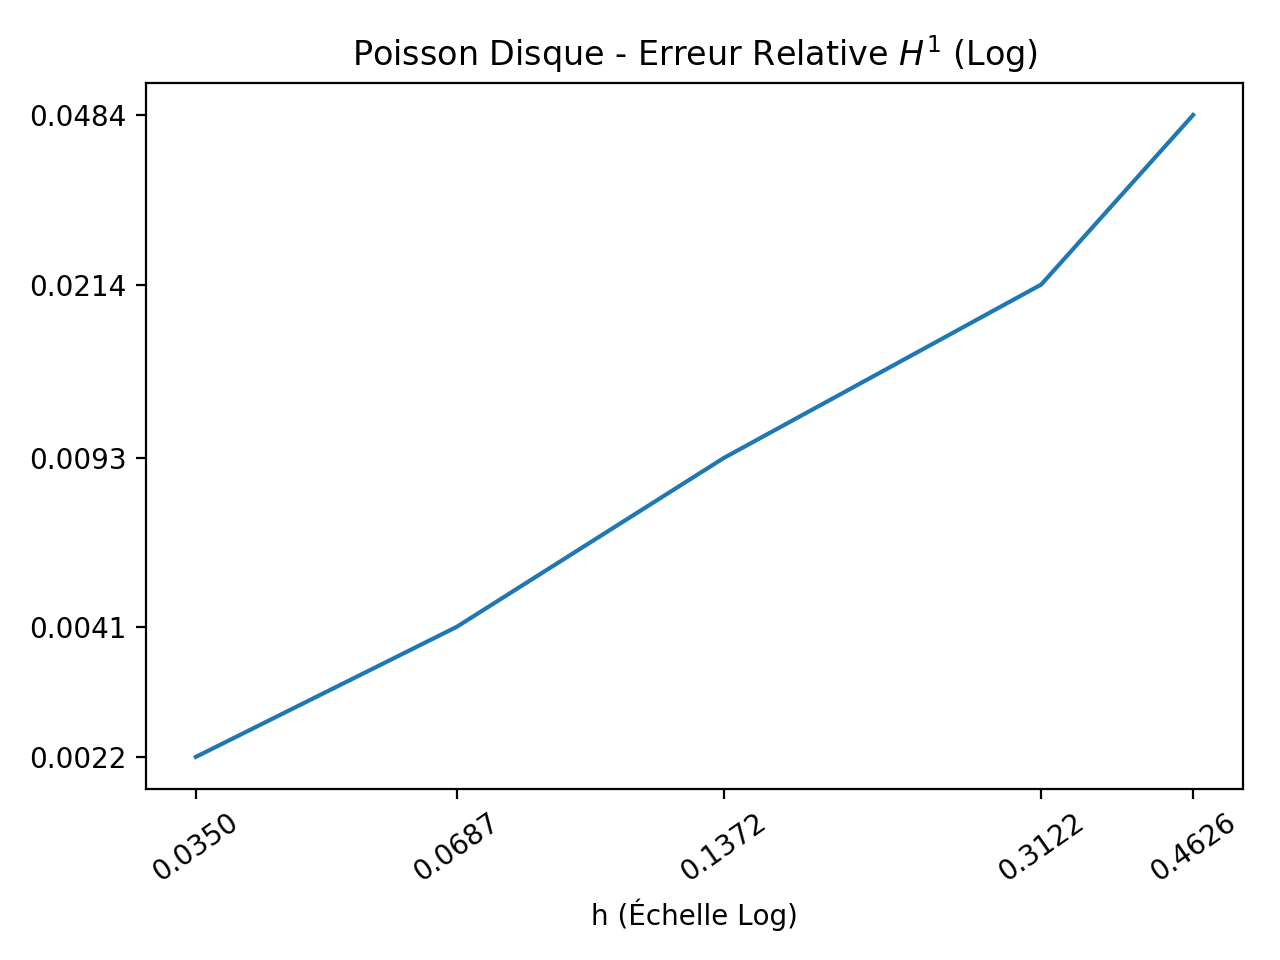
\includegraphics[scale=0.6]{figure_6.png}
\end{figure}

% ==============================================================================

\section*{Question 7}

On aimerait écrire le problème suivant sous forme variationnelle :

\[
\begin{dcases}
-\Delta u = 0 \text{ dans } \ouvert \\
u = g \text{ sur } \Gamma \\
\text{où } f \in C^\infty(\mathbb{R}^2)
\end{dcases}
\]

On suppose que $u \in C^2(\ouvert)$ et on se donne $v \in C^1(\ouvert)$.
Ensuite on multiplie l'égalité par $v$ et on l'integre. Cela nous donne
\[
-\int_\ouvert v \Delta u \; dx = \int_\ouvert vf \; dx
\]

Comme $u \in C^2(\ouvert)$ et $v \in C^1(\ouvert)$ on peut donc se
servir d'une formule de Green, ce qui nous améne à
\[
\int_\ouvert \nabla u \cdot \nabla v \; dx
- \int_\Gamma v \partial_{\bm n}{u} \; d\sigma = 0
\]

Avec $\lambda = \partial_{\bm n}{u}$ on a
\[
\int_\ouvert \nabla u \cdot \nabla v \; dx
+ \int_\Gamma \lambda v \; d\sigma = 0
\]

On multiplie la condition aux limites par une fonction $\mu \in L^2(\Omega)$
et l'integre pour arriver à
\[\int_\Gamma u \mu \; d\sigma = \int_\Gamma g \mu \; d\sigma\]

Comme $C^1(\ouvert)$ est dense dans $H^1(\ouvert)$ on suppose maintenant
que $u \in H^1(\ouvert)$. Par passage à la limite on en tire la formulation
variationnelle suivante :
\begin{eqnarray}
\int_\ouvert \nabla u \cdot \nabla v \; dx
+ \int_\Gamma \lambda v \; d\sigma = 0 & \forall v \in H^1(\ouvert) \\
\int_\Gamma u \mu \; d\sigma = \int_\Gamma g \mu \; d\sigma &
\forall \mu \in L^2(\Omega)
\end{eqnarray}

% ==============================================================================

\section*{Question 8}

On exprime $u_h$, $\lambda_h$, $v$ et $\mu$ dans la base de fonctions de forme :
\begin{align}
u_h &= \sum_{k=1}^{N_\Omega} u_k \phi_k^\Omega \\
\lambda_h &= \sum_{j=1}^{N_\Gamma} \lambda_j \phi_j^\Gamma \\
v &= \phi_j^\Omega \;\;\;\; j = 1 \sdots N_\Omega \\
\mu &= \phi_j^\Gamma \;\;\;\; j = 1 \sdots N_\Gamma
\end{align}

Cela nous amène à la formulation variationnelle discrète suivante :

Trouver $u_i$ ($i = 1 \sdots N_\Omega$) et $\lambda_j$ ($j = 1 \sdots N_\Gamma$)
telles que
\begin{eqnarray}
\int_\ouvert \nabla (\sum_{k=1}^{N_\Omega} u_k \phi_k^\Omega)
\cdot \nabla (\phi_j^\Omega) \; dx
%
+ \int_\Gamma (\sum_{k=1}^{N_\Gamma} \lambda_k \phi_k^\Gamma) (\phi_j^\Omega) \;
d\sigma = 0 & \forall j = 1 \sdots N_\Omega \\
%
\int_\Gamma (\sum_{j=1}^{N_\Omega} u_j \phi_j^\Omega) (\phi_k^\Gamma) \; d\sigma
= \int_\Gamma g \phi_k^\Gamma \; d\sigma &
\forall k = 1 \sdots N_\Gamma
\end{eqnarray}

En réarrangeant les termes de ces deux expressions on en tire
\begin{eqnarray}
\sum_{k=1}^{N_\Omega} u_k \int_\ouvert \nabla \phi_j^\Omega
\cdot \nabla \phi_k^\Omega \; dx
%
+ \sum_{k=1}^{N_\Gamma} \lambda_k \int_\Gamma \phi_j^\Omega \phi_k^\Gamma \;
d\sigma = 0 & \forall j = 1 \sdots N_\Omega \\
%
\sum_{j=1}^{N_\Omega} u_j \int_\Gamma \phi_k^\Gamma \phi_j^\Omega \; d\sigma
= \int_\Gamma g \phi_k^\Gamma \; d\sigma &
\forall k = 1 \sdots N_\Gamma
\end{eqnarray}

Or, avec $U$ le vecteur des composants $u_j$ ($j = 1 \sdots N_\Omega$) et
$L$ le vecteur des composants $\lambda_k$ ($k = 1 \sdots N_\Gamma$), on arrive
aux deux systèmes linéaires suivants :
\begin{eqnarray}
AU + BL = 0 \\
B^T U = G
\end{eqnarray}

Où
\begin{alignat}{2}
A_{j,k} &= \int_\ouvert \nabla \phi_j^\Omega \cdot \nabla \phi_k^\Omega \; dx &
j,k = 1 \sdots N_\Omega\\
%
B_{j,k} &= \int_\Gamma \phi_j^\Omega \phi_k^\Gamma \; d\sigma &
j = 1 \sdots N_\Omega, k = 1 \sdots N_\Gamma \\
%
G_k &= \int_\Gamma g \phi_k^\Gamma \; d\sigma & k = 1 \sdots N_\Gamma
\end{alignat}

Finalemenet, on combine ces deux systèmes en un seul systéme linéaire des matrices blocs :
\[
\begin{bmatrix}
  A & B \\
  B^T & 0
\end{bmatrix}
\begin{bmatrix}
  U \\
  L
\end{bmatrix} =
\begin{bmatrix}
  0 \\
  G
\end{bmatrix}
\]

% ==============================================================================

\section*{Question 9}

\paragraph{Exécuter le code :}
\begin{verbatim}
  ./question.sh 9
\end{verbatim}

\paragraph{Le code se trouve dans}
\begin{verbatim}
  questions/q9_verifier_solution_bloc.py
\end{verbatim}

\begin{figure}[H]
\centering
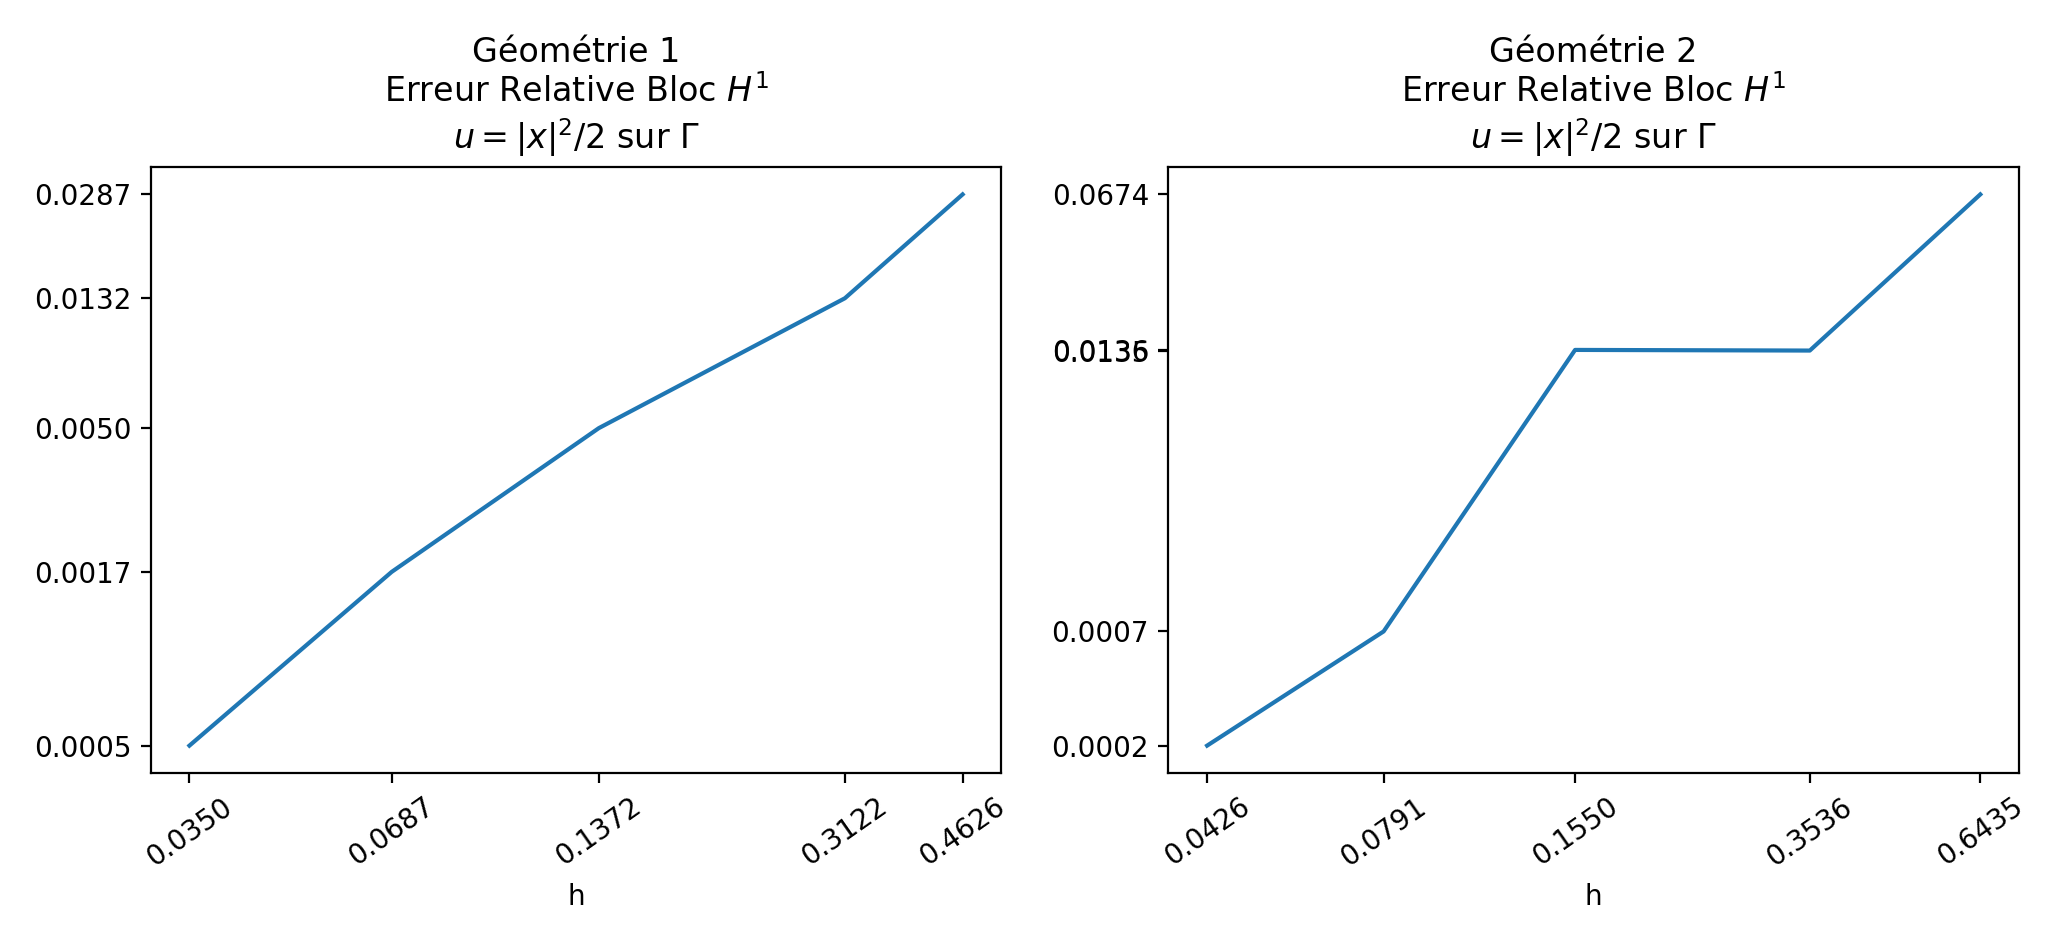
\includegraphics[scale=0.55]{figure_9.png}
\end{figure}

% ==============================================================================

\end{document}
